% \chapter[Signal]{Signal}

\section{Le signal de RMN}
La "mécanique" de l'aimantation décrite dans les paragraphes précédents montre
comment un échantillon dans son état d'équilibre magnétique est excité par une
impulsion de radio-fréquence et comment il revient vers son état initial en un
mouvement de précession de Larmor "amorti" par la relaxation.
L'utilisation de la RMN comme outil analytique nécessite la détermination
expérimentale du mouvement de l'aimantation.
Des résultats de cette mesure apparaissent les caractéristiques des
différentes populations de noyaux contenus dans l'échantillon.

La "bobine" qui transmet l'impulsion de courant de radiofréquence est à son
tour le siège d'une tension électrique alternative due au mouvement de
l'aimantation de l'échantillon.
Cette tension est appelée tension induite.
Dans un alternateur une partie mobile aimantée (rotor) tourne dans un
enroulement conducteur fixe (stator);
c'est très exactement de qui se passe en RMN où l'aimantation de l'échantillon
est mobile par rapport à la bobine fixe.
lorsque la bobine n'est plus utilisée pour transmettre
l'impulsion de radio-fréquence, la tension induite notée $e(t)$ est
enregistrée et analysée.
La tension induite est une grandeur physique mesurable dépendante du temps
définie pour $t \ge 0$,
l'instant $t = 0$ étant celui du début de son enregistrement.
L'expression "signal de RMN" ou "{\FIDfull}" ou "{\FID}"
(Free induction decay) désignera la fonction $e(t)$.

L'axe $Ox$ du référentiel du laboratoire a été choisi comme axe de la bobine au
paragraphe \ref{sec:macro}.
Le signal e(t) est créé par la variation de la projection de $\aimxs$ sur cet axe $Ox$ :
\begin{equation}
e(t) = K \derivt{\aimxs}
\end{equation}

Le nombre $K$ englobe un ensemble de facteurs géométriques liés à l'échantillon et à la
bobine, ainsi qu'un facteur lié au fait que la bobine est insérée dans
un circuit oscillant, circuit caractérisé par son facteur de surtension.
L'expression de $\aimxs(t)$ est
\begin{equation}
\aimxs(t) = A \cos(\omega_0 t + \phi) \exp(-t/T_2^*)
\end{equation}
dans l'hypothèse où un seul type de noyau est sollicité par l'impulsion de radio-fréquence.
Le facteur $A$ incorpore la valeur de l'aimantation d'équilibre $\aimzeros$ et le
facteur $\sin(\theta)$, où $\theta$ est l'angle de nutation (voir équation \ref{eqn:pulseaction}).
L'expression de $e(t)$ s'en déduit par dérivation :
\begin{equation}
e(t) = K A \exp(-t/T_2^*) (\omega_0 \sin(\omega_0 t + \phi) -
1/T_2^* \cos(\omega_0 t + \phi) )
\end{equation}

$e(t)$ est la somme de deux fonctions sinusoïdales amorties, l'une proportionnelle à
$\omega_0$, et l'autre à $1/T_2^*$, de plusieurs ordres de grandeur
inférieur à la première.
Le second terme est toujours négligeable devant le premier et donc :

\begin{equation}
e(t) = \emax \exp(-t/T_2^*) \sin(\omega_0 t + \phi)
\end{equation}

Formellement le signal $e(t)$ et l'aimantation $\aimxs(t)$ ont des expressions identiques,
à une différence de phase près.
Ces deux grandeurs seront souvent confondues par la suite bien qu'en réalité la première soit
la dérivée de la seconde par rapport au temps.
Ceci n'est possible qu'à cause de la
relative lenteur du phénomène de relaxation par rapport à la précession et à cause du
caractère sinusoïdal du signal.

Le paramètre le plus aisément modifiable par
l'expérimentateur est l'angle de l'impulsion de radiofréquence qui donne naissance au signal.
La composante horizontale $\aimxys$ de $\aimvec$ est maximale lorsque l'angle de l'impulsion est de
$\pi / 2$ ($\sin\theta=1$).
C'est donc à cette condition que l'amplitude du signal sera maximale,
en considérant que le signal ne provient que d'une seule séquence
impulsion--acquisition.
Dans une situation réelle où le rapport signal sur bruit est amélioré par
répétition de la séquence, il faut tenir compte de la vitesse de retour
de l'aimantation vers l'équilibre (donc des temps de relaxation) pour
choisir un angle de nutation optimal, angle qui est inférieur à $\pi/2$.

\section{Un récepteur très simplifié}
\label{sec:recept}

Toutes les fonctions d'un spectromètre par
impulsions et transformée de Fourier sont sous le contrôle d'un calculateur.
Cette nécessité s'est imposée par la nature de la chaîne de traitements qu'il faut faire subir au
signal $e(t)$ pour obtenir un spectre.
Un ensemble de traitements, comme l'amplification
et la démodulation (voir ci-après) sont du ressort de l'électronique analogique.

Le signal $e(t)$ a une fréquence égale à la fréquence de résonance des noyaux considérés,
qui se compte généralement en dizaines ou centaines de MHz.
S'il est techniquement
réalisable d'amplifier un tel signal (initialement de quelques $\mu$V), sa numérisation en
l'état n'est pas utile.

L'analyste désire en fait connaître la différence entre la fréquence de résonance des
noyaux étudiés et celle d'une substance de référence, différence qui donne accès aux
déplacements chimiques.
Ce qui est réalisé pratiquement par les circuits
électroniques de réception est une démodulation, opération qui
revient pratiquement à abaisser la fréquence du signal
d'une quantité égale à la fréquence des impulsions.
Le démodulateur livre un signal de basse fréquence $s(t)$ à partir du
signal $e(t)$ et de la tension délivrée par l'oscillateur qui pilote le générateur d'impulsion
(figure \ref{fig:spectroa}).
Le signal $s(t)$ est aussi appelé signal "audio--fréquence", par analogie à la
technique de réception radiophonique où le signal à transmettre est véhiculé par une
"onde porteuse" de haute fréquence puis démodulé (ou détecté) dans le récepteur.
A partir de
\begin{equation}
e(t) = A \exp(-t/T_2^*) \sin(\omega_0 t + \phi)
\end{equation}
le démodulateur fournit le signal $s(t)$ :
\begin{equation}
s(t) = A \exp(-t/T_2^*) \sin((\omega_0-\omrf) t + \phi)
= A \exp(-t/T_2^*) \sin(\omzeros t + \phi)
\end{equation}
où $\omzeros$ désigne la pulsation du signal d'audio--fréquence et $A$ son amplitude.
Le démodulateur abaisse la fréquence tout en conservant la phase du signal.
Il est indispensable de conserver l'information de la phase du signal dans $s(t)$ pour assurer,
entre autres choses, la possibilité d'augmentation du rapport signal/bruit par
accumulation.

La figure \ref{fig:spectroa} montre bien que le signal de référence ($\nuref = \omrf/2\pi$)
sert à la fois pour l'excitation de l'échantillon (il doit pour ce faire être amplifié
pour que ceci se déroule dans le temps le plus court possible) et pour la démodulation
du signal provenant de la sonde (c'est-à-dire de la partie du spectromètre qui 
entoure l'échantillon), signal qui doit être amplifié avant toute opération.
Le signal audio--fréquence est ensuite échantillonné (section \ref{sec:echantillon})
et numérisé par un convertisseur analogique-numérique (analog--digital converter, ou ADC) 
avant d'être traité par un calculateur (section \ref{sec:ft}).

\begin{figure}[hbt]
\begin{center}
\begin{pspicture}(0,1)(8.5,10.5)
\psset{linewidth=0.05}
\psframe(5.5,7.475)(6,10.5)
\psframe(5,7)(6.5,7.525)
\pscircle(5.5,7.25){0.1}
\pscircle(6,7.25){0.1}
\rput(4.75,7.75){Sonde}
\psframe(0,5.5)(1,6.5)
\rput(0.5,6){$\nuref$}
\psframe(3,5.5)(4,6.5)
\pspolygon(3.25,5.75)(3.75,6)(3.25,6.25)
\rput(3.5,6.75){Ampli.}
\psframe(7,5.5)(8,6.5)
\pspolygon(7.25,5.75)(7.75,6)(7.25,6.25)
\rput(7.5,6.75){Préampli.}
\psframe(7,4)(8,5)
\psline(7.25,4.25)(7.75,4.75)
\psline(7.75,4.25)(7.25,4.75)
\rput(5.75,4.75){Démodulateur}
\psframe(7,2.5)(8,3.5)
\rput(7.5,3){ADC}
\psframe(5,1)(8.5,2)
\rput(6.75,1.5){Calculateur}
\psline{->}(1,6)(3,6)
\psline(4,6)(5,6)(5.5,6.5)
\psline{<->}(5.5,6.5)(5.5,7)
\psline[linestyle=dashed,dash=5pt 5pt](5.5,6.5)(6,6)
\psline(6,6)(7,6)
\psline(8,6)(8.5,6)
\psline{->}(2,4.5)(7,4.5)
\psline{<-}(8,4.5)(8.5,4.5)
\psline(2,6)(2,4.5)
\psline(8.5,4.5)(8.5,6)
\psline{->}(7.5,4)(7.5,3.5)
\psline{->}(7.5,2.5)(7.5,2)
\end{pspicture}
\caption{\label{fig:spectroa}
\small Spectromètre très simplifié.}
\end{center}
\end{figure}

Il est commode de considérer que le démodulateur permet d'observer l'aimantation de
l'échantillon dans le référentiel tournant. Un signal $s(t)$ de fréquence nulle correspond à
la présence de noyaux exactement "en résonance" : $\omega_0 = \omrf$ et $\omzeros = 0$.
Un signal $s(t)$ de fréquence positive est dû à un noyau de fréquence de résonance
plus élevée que celle des impulsions.

Le schéma de détection du signal qui vient d'être présenté a l'inconvénient de fournir un
signal $s(t)$ où le signe de $\omzeros$ est ambigu.
Pour s'en rendre compte il suffit de considérer un premier signal
\begin{equation}
s_1(t)=A.\cos(\omzeros t + \phi).\exp(-t/T_2^*).
\end{equation}
Un autre noyau de pulsation de résonance $\omrf-\omzeros$ donnera un
signal
\begin{eqnarray}
s_2(t) & = & A.\cos(-\omzeros t + \phi).\exp(-t/T_2^*) \\
& = & A.\cos(\omzeros t - \phi).\exp(-t/T_2^*).
\end{eqnarray}
Dans l'expression de ces deux signaux apparaissent la même pulsation $\omzeros$ et des phases
opposées.
La phase n'étant pas connue de façon absolue, le signe de $\omzeros$ n'est pas
déterminé.
Un remède possible à cet état de fait consiste à choisir la fréquence des
impulsions en étant sûr qu'elle est soit supérieure (ou inférieure) à toutes les fréquences
de résonances présentées par les noyaux de l'échantillon ayant subi l'effet de
l'impulsion.

\section{La détection en quadrature}
Il ressort de l'analyse précédente qu'un schéma de détection monocanale (à
l'aide d'un seul démodulateur) ne peut pas donner accès au signe de $\omzeros$.
La technique de détection du signal dite "en quadrature" utilise deux démodulateurs, 
figure \ref{fig:spectrob}.
un premier démodulateur livre le signal $s_x(t)$, 
identique au signal $s(t)$ du paragraphe précédent.
La tension issue du circuit déphaseur est celle de l'oscillation pilote déphasée de 90$^{\circ}$.
Elle alimente le second démodulateur pour fournir le signal $s_y(t)$.
Les démodulateurs sont sensibles à la phase du signal qui les pilote, en conséquence :
\begin{eqnarray}
s_x(t) & = & A . \cos(\omzeros t + \phi) . \exp(-t/T_2^*) \\
s_y(t) & = & A . \sin(\omzeros t + \phi) . \exp(-t/T_2^*)
\end{eqnarray}
Si on porte dans un plan $XOY$ l'évolution du vecteur $\OMvec$ tel que
\begin{equation}
\OMvec = s_x(t) . \ivec + s_y(t) . \jvec
\end{equation}
on constate que ce vecteur retrace très exactement le mouvement de l'aimantation $\aimxyvec$
dans le référentiel tournant.
Le signe de $\omzeros$ est alors discernable sans ambiguïté.
Le traitement ultérieur des signaux $s_x(t)$ et $s_y(t)$, considérés simultanément, résout le
problème de la discrimination du signe de $\omzeros$.
Tout cela pour dire qu'il n'est pas possible de connaître le sens de rotation d'un objet
à partir de l'observation d'une seule projection de son mouvement et qu'il faut
deux projections pour y arriver.
Une manière commode de représenter le signal est de considérer la quantité complexe
\begin{equation}
s(t) = s_x(t) + is_y(t)
\end{equation}
qui contient toute l'information disponible sur l'aimantation transversale, à la
manière de $\OMvec$ mais en étant une quantité scalaire qui peut aussi s'écrire
\begin{equation}
\label{signalcomplexe}
s(t) = A . \exp(i(\omzeros t + \phi)) . \exp(-t/T_2^*)
\end{equation}
Le plan XOY du référentiel tournant est alors confondu avec le plan complexe comme 
l'indique la figure \ref{fig:xyplane}.

\begin{figure}[hbt]
\begin{center}
\begin{pspicture}(-4,-2)(4,2)
\SpecialCoor
\rput(-2.5,0){
\psline{->}(-1.5,0)(1.5,0)
\uput[0](1.5,0){$X$}
\psline{->}(0,-1.5)(0,1.5)
\uput[90](0,1.5){$Y$}
\uput[-135](0,0){$O$}
\psline{->}(0,0)(1,0)
\uput[-90](1,0){$\boldsymbol{\vec{\imath}}$}
\psline{->}(0,0)(0,1)
\uput[180](0,1){$\boldsymbol{\vec{\jmath}}$}
\psline[linewidth=0.05]{->}(0,0)(1.2;60)
\uput{2pt}[60](1.2;60){$\boldsymbol{\vec{M}}$}
}
\rput(2.5,0){
\psline(-1.5,0)(1.5,0)
\uput[0]{-90}(1.5,0){Réel}
\psline(0,-1.5)(0,1.5)
\uput[90]{0}(0,1.5){Imaginaire}
\uput[-135](0,0){$0$}
\psline(1,-0.1)(1,0.1)
\uput[-90](1,0){$\boldsymbol{1}$}
\psline(-0.1,1)(0.1,1)
\uput[180](0,1){$\boldsymbol{i}$}
\psline[linewidth=0.05]{->}(0,0)(1.2;60)
\uput{2pt}[60](1.2;60){$\boldsymbol{M}$}
}
\end{pspicture}
\caption{\label{fig:xyplane}
\small Plan transversal du référentiel tournant et plan complexe.}
\end{center}
\end{figure}

Une autre réalisation pratique de la
détection en quadrature est due à Redfield, mais le détail de son fonctionnement
nécessite la connaissance de l'échantillonnage du signal.

\begin{figure}[hbt]
\begin{center}
\begin{pspicture}(0,0)(8.5,10.5)
\psset{linewidth=0.05}
\psframe(5.5,7.475)(6,10.5)
\psframe(5,7)(6.5,7.525)
\pscircle(5.5,7.25){0.1}
\pscircle(6,7.25){0.1}
\rput(4.75,7.75){Sonde}
\psframe(0,5.5)(1,6.5)
\rput(0.5,6){$\nuref$}
\psframe(3,5.5)(4,6.5)
\pspolygon(3.25,5.75)(3.75,6)(3.25,6.25)
\rput(3.5,6.75){Ampli.}
\psframe(7,5.5)(8,6.5)
\pspolygon(7.25,5.75)(7.75,6)(7.25,6.25)
\rput(7.5,6.75){Préampli.}
\psframe(7,4)(8,5)
\psline(7.25,4.25)(7.75,4.75)
\psline(7.75,4.25)(7.25,4.75)
\rput(5.75,4.75){Démodulateur}
\psframe(5.5,3)(6.5,4)
\psline(5.75,3.25)(6.25,3.75)
\psline(6.25,3.25)(5.75,3.75)
\psframe(2.5,3)(4.5,4)
\rput(3.5,3.5){$\Delta\phi=90^{\circ}$}
\rput(3.5,2.75){Déphaseur}
\psframe(5.5,1.5)(6.5,2.5)
\rput(6,2){ADC}
\psframe(7,1.5)(8,2.5)
\rput(7.5,2){ADC}
\psframe(5,0)(8.5,1)
\rput(6.75,0.5){Calculateur}
\psline{->}(1,6)(3,6)
\psline(4,6)(5,6)(5.5,6.5)
\psline{<->}(5.5,6.5)(5.5,7.25)
\psline[linestyle=dashed,dash=5pt 5pt](5.5,6.5)(6,6)
\psline(6,6)(7,6)
\psline(8,6)(8.5,6)
\psline{->}(2,4.5)(7,4.5)
\psline{<-}(8,4.5)(8.5,4.5)
\psline{->}(2,6)(2,3.5)(2.5,3.5)
\psline{->}(4.5,3.5)(5.5,3.5)
\psline{<-}(6.5,3.5)(7.3,3.5)
\psline(7.7,3.5)(8.5,3.5)(8.5,6)
\psline{->}(6,3)(6,2.5)
\psline{->}(6,1.5)(6,1)
\psline{->}(7.5,4)(7.5,2.5)
\psline{->}(7.5,1.5)(7.5,1)
\end{pspicture}
\caption{\label{fig:spectrob}
\small Spectromètre utilisant la détection en quadrature.}
\end{center}
\end{figure}

\section{L'échantillonneur}
\label{sec:echantillon}
Le signal est une grandeur qui varie continûment au cours du temps.
Pour être traité par un calculateur numérique il faut l'échantillonner,
c'est à dire ne retenir du signal s(t)
qu'un nombre discret de valeurs (échantillons...), mesurées à des instants régulièrement
espacées.
Une "image" du signal est ainsi crée qui est d'autant plus fidèle au signal
d'origine que la fréquence des mesures est élevée.
En contrepartie, il y aura plus de valeurs de mesure à traiter et à stocker.
De plus, l'échantillonnage est d'autant plus délicat à
réaliser que sa fréquence est rapide.
A partir de la fonction $s(t)$ on construit une suite de
valeurs de tension $s_n$ telle que
\begin{equation}
s_n = s(n . \Delta t)
\end{equation}
où $n$ est le numéro de l'échantillon et $\Delta t$ le temps qui sépare deux mesures.
Les tensions $s_n$ sont ensuite converties en nombres binaires
par un convertisseur analogique-digital,
étape indispensable au traitement informatisé du signal.
Un grand nombre $N$ d'échantillons est ainsi mesuré,
$N$ étant généralement une puissance de 2.
L'inverse du temps qui sépare deux mesures définit la fréquence d'échantillonnage :
\begin{equation}
\nuech = \frac{1}{\Delta t}
\end{equation}
qui est le nombre de mesures effectuées en une seconde.
Le choix de $\nuech$ est déterminé par la
plus grande valeur de fréquence présente dans le signal, notée $\numax$ :
\begin{equation}
- \numax  < \frac{\omzeros}{2\pi} < + \numax
\end{equation}
Le théorème de Nyquist affirme qu'il faut que
\begin{equation}
\nuech = 2 . \numax
\end{equation}
Cela se justifie en considérant les signaux numérisés issus de deux signaux sinusoïdaux
de fréquence $\numax - \delta\nu$ et $\numax + \delta\nu$.
Un signal $s(t) = \cos(\omega t + \phi)$ se numérise en
$s_n = \cos(2\pi\nu n/2\numax + \phi)$ puisque $\Delta t = 1/2\numax$.

Si $\nu = \numax - \delta\nu$ alors
\begin{eqnarray}
s_n & = & \cos(2\pi n (\numax - \delta\nu)/2\numax + \phi) \\
& = & \cos(\pi n(1-\delta\nu/\numax) + \phi)
\end{eqnarray}

Si $\nu = \numax + \delta\nu$ alors
\begin{eqnarray}
s_n & = & \cos(2\pi n (\numax + \delta\nu)/2\numax + \phi) \\
& = & \cos(\pi n(1+\delta\nu/\numax) + \phi) \\
& = & \cos(\pi n(-1-\delta\nu/\numax) - \phi) \\
& = & \cos(2\pi n + \pi n(-1-\delta\nu/\numax) - \phi) \\
& = & \cos(\pi n(1-\delta\nu/\numax) - \phi)
\end{eqnarray}

\begin{figure}[hbt]
\begin{center}
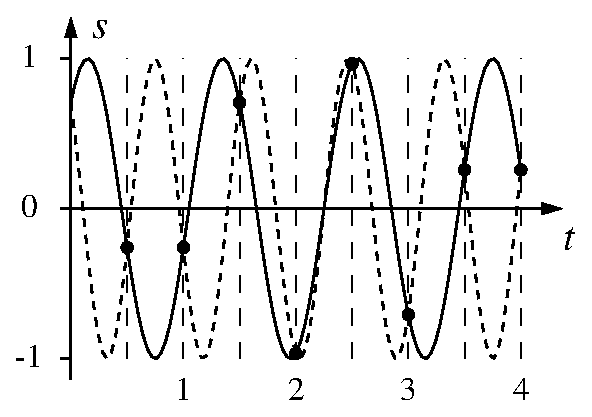
\epsfig{file=alias.eps,width=3in}
\end{center}
\caption{Illustration du phénomène de repliement spectral.}
\label{fig:aliasing}
\end{figure}

puisque $\cos(x+2\pi n) = \cos(x)$ et $\cos(x) = \cos(-x)$.
Les signaux numérisés sont donc indiscernables du point de vue de leur fréquence.
Un raisonnement général indique que tous les signaux de
fréquence $\nu$ tels que $\nu > \numax$ et $\nu < -\numax$ peuvent être considérés
après échantillonnage comme des signaux de fréquence comprise entre $-\numax$ et $+\numax$,
entraînant l'apparition d'informations erronées.
Ce phénomène porte le nom de
repliement spectral et est illustré figure \ref{fig:aliasing} 
où deux signaux de fréquences $\numax - \delta\nu$ et
$\numax + \delta\nu$ prennent des valeurs identiques à tous les instants d'échantillonnage.
Dans cette figure, $\numax = 1$ Hz et donc $\nuech = 2$ Hz, ce qui conduit à une
prise d'échantillons toutes les 0.5 s, matérialisée par les traits verticaux en pointillés fins
et les cercles.
Les signaux  représentés ont pour fréquence $1 - 1/6$ Hz (en trait plein) et
$1 + 1/6$ Hz (en pointillé). Leur échantillonnage conduit exactement
aux même mesures, ce qui prouve qu'ils seront vus de la même manière par
les traitement ultérieurs et conduiront à des spectres identiques.

Le cas qui vient d'être traité correspond à une détection du signal sur un seul canal,
cas dans lequel des signaux de fréquences opposés sont indiscernables.
La bande spectrale utile ne s'étend alors que de la fréquence 0 à la fréquence $\numax$,
soit une largeur spectrale de $\numax$.
La fréquence d'échantillonnage doit alors être le double de la largeur spectrale.
Dans le cas de la détection du signal complexe, la largeur spectrale $2\numax$ est égale
à la fréquence d'échantillonnage $2\numax$.
Deux signaux complexes de fréquences $\nu$ et $\nu+2\numax = \nu+\nuech$ sont 
en effet échantillonnés identiquement :
\begin{eqnarray}
s_n & = & \exp(i(2 \pi n (\nu + \nuech)/\nuech + \phi)) \\
& = & \exp(i(2 \pi n \nu/\nuech + 2 \pi n + \phi)) \\
& = & \exp(i(2 \pi n \nu/\nuech)).\exp(2 i \pi n) \\
& = & \exp(i(2 \pi n \nu/\nuech))
\end{eqnarray}.

Les signaux issus du repliement spectral 
sont de deux natures : il s'agit soit de signaux vrais 
(issus de l'échantillon) de fréquence trop
élevée soit de composantes du bruit de fond.
Un filtre dit "filtre audio" placé entre le démodulateur et l'échantillonneur
et dont la bande passante est légèrement supérieure à la largeur spectrale
voulue atténue ces signaux indésirables.

Les spectromètres modernes utilisent la technique du sur-échantillonnage dans
laquelle $\nuech$ est beaucoup plus grand que requis par le critère de Nyquist.
Le filtrage est alors réalisé par une technique numérique et non plus
par des composants analogiques.

\section{Le "Redfield trick"}
\label{sec:redfield}

Les signaux $s_x(t)$ et $s_y(t)$ issus du double démodulateur décrit figure
\ref{fig:spectrob} sont soit
échantillonnés simultanément (pour former le signal complexe), 
et on parlera de détection simultanée, soit échantillonnés
séquentiellement selon la méthode de Redfield.
Un système d'aiguillage électronique permet en fait de n'utiliser 
qu'un seul démodulateur et qu'un seul convertisseur, même pour
la détection simultanée.

Dans le cas de la détection séquentielle,
un seul signal réel est construit à partir de $s_x(t)$ et de $s_y(t)$
en intercalant un échantillon de $s_x(t)$ avec un de
$s_y(t)$ puis en changeant le signe des valeurs mesurées.
En supprimant comme au paragraphe précédent le terme
d'amplitude et de relaxation qui n'apportent rien à la compréhension de la méthode,
à partir de $s_x(t) = \cos(\omzeros t + \phi)$ et de $s_y(t) = \sin(\omzeros t + \phi)$
le signal échantillonné $s_n$ est tel
que :
\begin{eqnarray}
s_0 & = & +s_x(0 . \Delta t) = +\cos(\omzeros.0.\Delta t + \phi) \\
s_1 & = & -s_y(1 . \Delta t) = -\sin(\omzeros.1.\Delta t + \phi) \\
s_2 & = & -s_x(2 . \Delta t) = -\cos(\omzeros.2.\Delta t + \phi) \\
s_3 & = & +s_y(3 . \Delta t) = +\sin(\omzeros.3.\Delta t + \phi) \\
s_4 & = & +s_x(4 . \Delta t) = +\cos(\omzeros.4.\Delta t + \phi) \\
\mbox{etc...} & &
\end{eqnarray}
L'expression de $s_0$ .... $s_4$ se réécrit  :
\begin{eqnarray}
s_0 =  \cos(\omzeros.0.\Delta t + 0 . \pi/2 + \phi) \\
s_1 =  \cos(\omzeros.1.\Delta t + 1 . \pi/2 + \phi) \\
s_2 =  \cos(\omzeros.2.\Delta t + 2 . \pi/2 + \phi) \\
s_3 =  \cos(\omzeros.3.\Delta t + 3 . \pi/2 + \phi) \\
s_4 =  \cos(\omzeros.4.\Delta t + 4 . \pi/2 + \phi) \\
\mbox{etc...} & &
\end{eqnarray}
Si $\Delta t$ est choisi maintenant comme $1/4\numax$, c'est-à-dire si la fréquence
d'échantillonnage est double de celle utilisée en détection simultanée, 
le signal $s(t)$ qui
donnerait $s_n$ une fois échantillonné s'écrit en remplaçant $n$ par $t/\Delta t$.
\begin{eqnarray}
s(t) & = & \cos(2\pi\nu_0 t + t.4\numax.\pi/2 + \phi) \\
     & = & \cos(2\pi(\nu_0 + \numax)t + \phi)
\end{eqnarray}
On constate que ceci revient à augmenter la phase $\phi$ d'une quantité
proportionnelle au temps.
Puisque $\numax$ est par définition la fréquence la plus élevée du signal,
la quantité $\nu_0 + \numax$ est toujours positive.
Le signal $s(t)$ construit par la méthode de Redfield ne
contient que des signaux de fréquence positive et le problème de la détermination du
signe de $\nu_0$ (ou de $\omzeros$) ne se pose plus.
Lorsque la fréquence des impulsions est choisie
de façon à ce que les signaux $s_x(t)$ et $s_y(t)$ aient une fréquence comprise entre
$-\numax$ et $+\numax$,
(on dira : "la porteuse est au milieu du spectre") la méthode de "préparation" de
$s(t)$ décale toutes les fréquences de la quantité $\numax$.
Le critère de Nyquist impose donc le
doublement de la fréquence d'échantillonnage ($\Delta t = 1/4\numax$) puisque les fréquences
intervenant dans $s(t)$ sont comprises entre 0 et $2.\numax$.

La façon dont $s(t)$ est construit par la méthode de Redfield
est en fait une mesure de $\aimvec$ sur un axe $OR$ mobile par
rapport au référentiel tournant.
$\aimvec$ est successivement mesuré sur les axes :
\begin{eqnarray}
+OX		& \mbox{au temps} &		0 \\
-OY		& &			1/4\numax \\
-OX		& &			2/4\numax \\
+OY		& &			3/4\numax \\
+OX		& &			4/4\numax \\
\mbox{etc...}& &
\end{eqnarray}
L'axe $OR$ sur lequel $\aimvec$ est mesuré fait donc un tour en un temps $4/4\numax$,
sa fréquence de rotation par rapport au référentiel tournant est donc $\numax$,
dans le sens négatif de rotation.
Tout vecteur tournant à une fréquence $\nu$ supérieure à $-\numax$ par rapport au
référentiel tournant (cela doit être le cas de tous les vecteurs $\aimvec$) apparaîtra 
bien comme
tournant à une fréquence positive par rapport à l'axe OR.

\section{Analyse harmonique et linéarité}
\label{sec:ft}
Après démodulation en quadrature et échantillonnage le spectromètre délivre soit un 
ensemble de signaux $s_x(t)$ et $s_y(t)$ sous forme d'un signal complexe
si la détection est simultanée soit un signal réel unique $s(t)$ 
si la méthode de détection de Redfield est employée. 
Ces signaux proviennent du retour 
à l'équilibre d'un ensemble de noyaux préalablement excités par une impulsion de 
radio-fréquence. 
La  question à résoudre par l'analyste est : combien de type de noyaux résonnent à quelle 
fréquence? 
Répondre à cette question revient à élaborer un graphique portant en 
abscisse des fréquences et en ordonnée une amplitude qui caractérise le nombre de 
noyaux résonnant à chaque fréquence. 
Un tel graphique est un spectre, représentation 
d'une fonction notée $S(\Oms)$. 
Le but de l'analyse harmonique est la transformation d'un 
signal $s(t)$, fonction du temps, 
en une fonction de la pulsation (ou de la fréquence) $S(\Oms)$ 
qui caractérise le "contenu sinusoïdal" du signal.

Jusqu'ici seul des ensembles de noyaux identiques ont été considérés pour établir 
l'expression de $e(t)$, $s(t)$ et $s_n$. 
Ces noyaux sont caractérisés par leur pulsation 
propre $\omzeros$, leur temps de relaxation transversal apparent $T_2^*$, 
et leur aimantation initiale $\aimzerovec$. 
Les opérations qui mènent de $\aimvect$ à $s_n$ sont linéaires (si elles sont effectivement 
réalisées de façon idéale) c'est à dire que le résultat ($s_n$) obtenu en considérant plusieurs 
populations de noyaux est celui qui serait obtenu en faisant la somme des résultats 
individuels obtenus à partir des différentes populations prises séparément. 
Plus formellement une opération $O$ qui agit sur deux objets $x_1$ et $x_2$ 
(vecteurs, fonctions...) est linéaire si :
\begin{eqnarray}
O(x_1 + x_2) & = & O(x_1) + O(x_2) \\
O(\lambda . x_1) & = & \lambda . O(x_1)
\end{eqnarray}
L'aimantation totale d'un ensemble de deux noyaux est la somme de leurs aimantations 
individuelles. 
Sous réserve que l'impulsion soit non sélective, l'amplitude de 
l'aimantation transversale se déduit de l'angle de nutation de 
l'impulsion de façon identique pour les 
différentes populations de noyaux. 
Le passage de l'aimantation 
transversale vers le signal $e(t)$ fait intervenir une dérivation par rapport au temps, 
opération qui est linéaire : la dérivée d'une somme de fonctions est la somme de leurs 
dérivées. 
Les étapes d'amplification, de démodulation et d'échantillonnage sont linéaires 
dans la mesure où leur réalisation pratique est infiniment parfaite... 
Fondamentalement la conversion analogique-numérique est nécessairement une étape non linéaire 
puisqu'un il faut que le signal atteigne au moins une valeur de seuil (non nulle) pour 
que le convertisseur donne autre chose que la valeur numérique nulle. 
D'un point de vue pratique la "numérisation" du signal est considérée comme linéaire 
si la valeur de seuil est très faible,
c'est-à-dire si la taille du nombre binaire fournie est grande. 

L'opération qui transforme le signal numérisé en spectre numérisé est une opération 
linéaire, réalisée par différentes méthodes de calcul numérique. 
Parmi ces méthodes la Transformation de Fourier est actuellement la plus répandue, 
essentiellement à cause de sa très grande vitesse d'exécution. 
La linéarité de la transformation de Fourier nous autorise à poursuivre le 
cheminement du signal en ne considérant qu'une seule population de noyaux identiques.

\section{La transformation de Fourier (TF) réelle}
Appliquer la transformation de Fourier réelle (réelle, par opposition à complexe) à un 
signal, c'est faire implicitement l'hypothèse que ce signal est une fonction du temps à 
valeurs réelles qui s'écrit comme une somme de fonctions sinusoïdales d'amplitudes et de 
phases à déterminer pour chaque fréquence (ou pulsation) possible. 
Dans un cas général il ne s'agit pas d'une somme 
discrète mais d'une superposition continue de sinusoïdes :
\begin{equation}
s(t) = \intmp A(\Oms) \cos(\Oms t + \phi(\Oms)) \, d\Oms
\end{equation}
Une sinusoïde amortie, par exemple, ne peut pas en toute rigueur s'écrire comme une 
somme de sinusoïdes pures en nombre fini. 
En développant l'expression de $s(t)$ sous la 
forme :
\begin{equation}
s(t) = \intzp R(\Oms) \cos\Oms t \, d\Oms + \intzp I(\Oms) \sin\Oms t \, d\Oms
\end{equation}
le terme de phase $\phi(\Oms)$ est englobé dans les fonctions $R(\Oms)$ et $I(\Oms)$. 
On peut montrer que : 
\begin{eqnarray}
\label{eqn:ftftr}
R(\Oms) & = & \intzp s(t).\cos \Oms t \, dt \\
\label{eqn:ftfti}
I(\Oms) & = & \intzp s(t).\sin \Oms t \, dt
\end{eqnarray}
en toute rigueur des facteurs multiplicatifs doivent figurer devant les expressions de 
$R(\Oms)$ et de $I(\Oms)$ mais ils n'apportent pas de modification au raisonnement. 
Une justification de ces expressions est donnée dans l'appendice \ref{chap:fourier}.

Dans un premier temps nous allons considérer que $s(t)$ provient de l'évolution libre d'un 
seul type de noyau et que le facteur de phase est nul : 
$s(t) = \cos \omzeros t . \exp(-t/\lambda_0)$. 
L'évaluation de $R(\Oms)$ et de $I(\Oms)$ s'obtient en calculant :
\begin{eqnarray}
R(\Oms) & = & \intzp  \cos\Oms t . \cos \omzeros t . \exp(-t/\lambda_0) \, dt \\
\mbox{et}\quad	
I(\Oms) & = & \intzp  \sin\Oms t . \cos \omzeros t . \exp(-t/\lambda_0) \, dt
\end{eqnarray}
Les calculs sont simplifiés en considérant que :
\begin{eqnarray}
\intzp \cos \Oms t . \exp(-t/\lambda_0) \, dt & = & \lambda_0/(1 + \lambda_0^2 \Oms^2) \\
\mbox{et}\quad
\intzp \sin \Oms t . \exp(-t/\lambda_0) \, dt & = & \Oms\lambda_0^2/(1 + \lambda_0^2 \Oms^2)
\end{eqnarray}
Sachant que
\begin{equation}
\cos \Oms . \cos \omzeros = \cos(\Oms - \omzeros) + \cos(\Oms + \omzeros), 
\end{equation}
à un facteur 2 près (sans importance) on déduit :
\begin{equation}
R(\Oms) = \lambda_0/(1 + (\Oms - \omzeros)^2\lambda_0^2) + 
\lambda_0/(1 + (\Oms + \omzeros)^2\lambda_0^2)
\end{equation}
Les deux termes sont semblables et changer $\omzeros$ en $-\omzeros$ 
donne la même valeur de $R(\Oms)$. 
La fonction
\begin{equation}
A(\Oms) = \lambda_0/(1 + (\Oms - \omzeros)^2\lambda_0^2)
\end{equation}
est appelée fonction de Lorentz  en absorption et sa représentation graphique, figure \ref{fig:absorp}, 
est la courbe lorentzienne $A(\Oms)$, centrée sur $\Oms = \omzeros$, ayant en ce point sa valeur maximale $\lambda_0$. 
Sa largeur à mi-hauteur vaut $2/\lambda_0$, elle est matérialisée par les points $A$ et $B$.
La fonction représentée est en fait $A(\Oms)/\lambda$ dont le maximum
est toujours égal à 1.

\begin{figure}[hbt]
\begin{center}
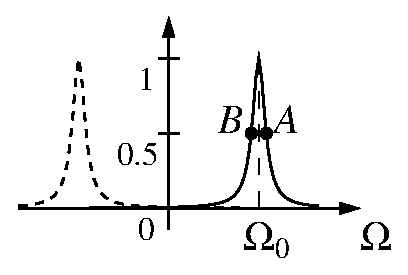
\epsfig{file=absorp.eps,width=2in}
\end{center}
\caption{\label{fig:absorp}Fonction de Lorentz (absorption).}
\end{figure}

Les fonctions de Lorentz centrées sur 
$\Oms = \omzeros$ seront notées $A(\omzeros)$, 
bien qu'il s'agisse implicitement d'une fonction de la variable $\Oms$ 
dont $\omzeros$ est un paramètre. 
Dans le cas étudié :
\begin{equation}
R(\Oms) = A(\omzeros) + A(-\omzeros)
\end{equation}
La courbe en pointillé sur la figure \ref{fig:absorp} est centrée autour
de $-\omzeros$ ; sa contribution à la partie du spectre où $\Oms \ge 0$ est pratiquement
négligeable.

Suivant des calculs analogues
\begin{eqnarray}
I(\Oms) & = & D(\omzeros) + D(-\omzeros) \\
\mbox{où}\quad D(\omzeros) & = & \lambda_0^2(\Oms - \omzeros)/
(1 + (\Oms - \omzeros)^2\lambda_0^2) 
\end{eqnarray}
La fonction $D(\Oms)$ est la fonction de Lorentz en dispersion.
Les représentations graphiques de $D(\Oms)/\lambda$ (trait plein)
et de $D(-\omzeros)/\lambda$ (trait pointillé) sont données 
figure \ref{fig:dispers}.
Les valeurs du maximum et du minimum sont respectivement 0.5 et -0.5 et leur
écartement en fréquence vaut $2/\lambda$.
La largeur à mi-hauteur est donc nécessairement plus grande que celle
de la courbe d'absorption.

\begin{figure}[hbt]
\begin{center}
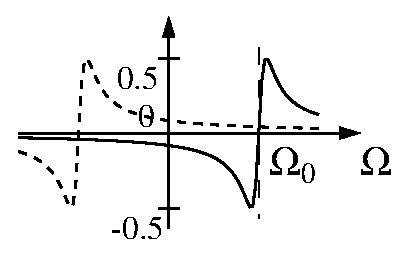
\epsfig{file=dispers.eps,width=2in}
\end{center}
\caption{\label{fig:dispers}Fonction de Lorentz (dispersion).}
\end{figure}

Les transformées de Fourier réelles $R(\Oms)$ et $I(\Oms)$ 
ne se calculent qu'à partir de signaux (réels) où toutes les 
fréquences sont censées être du même signe, puisqu'elles ne s'applique qu'à un seul 
signal (voir section \ref{sec:recept} et \ref{sec:redfield}).
On ne conserve généralement de $R(\Oms)$ et de $I(\Oms)$ que la partie 
correspondant aux fréquences positives. 
Dans la mesure où les raies spectrales ont une largeur faible par rapport à
la largeur spectrale totale et où les raies ne sont pas
trop proches des bords du spectres, les contributions de $A(-\omzeros)$ et de 
$D(-\omzeros)$ sont négligeables et on peut donc considérer que 
$R(\Oms) = A(\omzeros)$ et que $I(\Oms) = D(\omzeros)$,
ce qui est plus vrai pour $A(\Oms)$ que pour $D(\Oms)$, comme il
est possible de se rendre compte en comparant les figures
\ref{fig:absorp} et \ref{fig:dispers}, tracées avec des paramètres identiques.

Le spectre $S(\Oms)$ usuellement présenté à l'analyste est la représentation de la fonction 
$A(\Oms)$, dite courbe en Absorption pure. 
La fonction $D(\Oms)$ n'est en général pas 
représentée.
La fonction $D(\Oms)$ est en effet intrinsèquement plus large que $A(\Oms)$
ce qui rend plus difficile la distinction entre deux raies de fréquences proches,
entre autres inconvénients.

Dans l'exemple qui vient d'être traité, où la phase du signal est nulle, 
les fonctions $R(\Oms)$ et $A(\Oms)$ d'une 
part et $I(\Oms)$ et $D(\Oms)$ d'autre part sont identiques. 
Il n'en est pas de même lorsque la phase du signal n'est pas nulle. 
Pour obtenir un spectre où toutes les raies sont des 
courbes en absorption pure il faut nécessairement appliquer un
traitement à $R(\Oms)$ et $I(\Oms)$, le phasage.
Avant d'aborder cette question, regardons le sens physique du résultat qui vient d'être obtenu.

Un signal $s(t)$, produit d'une fonction sinusoïdale
de phase nulle et de pulsation $\omzeros$ par 
un facteur d'amortissement se décompose comme une somme d'une infinité de 
sinusoïdes de pulsations voisines de $\omzeros$. 
Moins ce signal est amorti, c'est-à-dire plus $\lambda_0$ est grand, 
et moins il y a de "participation" des sinusoïdes de fréquence éloignées de $\omzeros$ 
dans le signal. 
A l'extrême limite, si le signal est une sinusoïde pure, $S(\Oms)$ est 
une fonction nulle partout sauf pour $\Oms = \omzeros$ où elle prend une valeur infinie. 
La surface située sous la courbe en absorption ne dépend pas 
du facteur d'amortissement : diviser 
$\lambda_0$ par 2 double la largeur de la raie et divise par deux sa hauteur. 
La surface de la raie en absorption contient donc l'information quantitative 
que l'on peut tirer de la RMN : 
il est possible de tirer d'un spectre les populations relatives des différents types de noyaux 
de l'échantillon en faisant le rapport des surfaces des pics d'absorption correspondants. 
Les programmes de traitement des spectres permettent le calcul de ces surfaces relatives 
par intégration numérique de parties de spectres. 
Cela n'est pas le seul intérêt de la présentation des spectres en absorption : 
comme l'indiquent les figures \ref{fig:absorp} et \ref{fig:dispers}, les raies 
d'absorption sont, toutes choses égales par ailleurs, moins large que les raies en 
dispersion, amenant par là-même une sensible amélioration de la résolution des 
spectres. 
La présence de la fonction $I(\Oms)$ se justifie par la nature causale du signal : il 
n'est défini que pour $t \ge 0$ ; son calcul se justifie lorsqu'il y a lieu de phaser les spectre.

Si maintenant le signal contient un terme de phase : 
\begin{eqnarray}
s(t) & = & \cos (\omzeros t + \phi). \exp(-t/\lambda_0) \\ 
& = & \cos \omzeros t . \cos \phi . \exp(-t/\lambda_0) - 
\sin \omzeros t . \sin \phi . \exp(-t/\lambda_0)
\end{eqnarray}
le calcul de $R(\Oms)$ et de $I(\Oms)$ 
nécessite l'établissement des résultats suivants :
\begin{eqnarray}
\intzp  \cos \Oms t . \sin \omzeros t . \exp(-t/\lambda_0) \, dt & = &
D(\omzeros) - D(-\omzeros) \\
\mbox{et}\quad
\intzp  \sin \Oms t . \sin \omzeros t . \exp(-t/\lambda_0) \, dt & = &
A(\omzeros) - A(-\omzeros)
\end{eqnarray}
En ne gardant que la partie où $\Oms$ est positif dans $R(\Oms)$ et $I(\Oms)$ :
\begin{eqnarray}
R(\Oms) & = & A(\omzeros) . \cos \phi - D(\omzeros) . \sin \phi \\
\mbox{et}\quad 
I(\Oms) & = & A(\omzeros) . \sin \phi + D(\omzeros) . \cos \phi
\end{eqnarray}
La valeur de la phase étant a priori indéterminée $R(\Oms)$ et $I(\Oms)$ sont généralement des 
combinaisons de raies en absorption et en dispersion. 
Des spectres en absorption pure $S_A(\Oms)$ et $S_D(\Oms)$ sont calculables à partir de 
$R(\Oms)$ et de $I(\Oms)$ :
\begin{eqnarray}
S_A(\Oms) & = & R(\Oms) . \cos \phi + I(\Oms) . \sin \phi = A(\omzeros) \\
S_D(\Oms) & = & I(\Oms) . \cos \phi - R(\Oms) . \sin \phi = D(\omzeros)
\end{eqnarray}
Le spectre $S(\Oms)$ recherché est $S_A(\Oms)$, 
le spectre en dispersion pure est calculé pour 
permettre un phasage ultérieur si la valeur de $\phi$ choisie n'est pas correcte. 
La phase de tous les signaux issus d'un même échantillon serait identique si 
l'acquisition du signal commençait juste après l'impulsion. 
Cette commutation infiniment rapide n'est pas 
réalisable techniquement et un délai d'attente est nécessaire entre l'émission d'une 
impulsion et la réception du signal. 
Pendant ce délai les différentes composantes du 
signal se déphasent les unes des autres d'un angle égal au produit de leur pulsation par la 
durée du délai, ce qui aboutit à une dépendance linéaire entre $\phi$ et $\omzeros$ :
$\phi(\Oms) = a\Oms + b$.
L'opération qui consiste à trouver les paramètres $a$ et $b$ tels que 
$S_A(\Oms)$ ne présente que des raies en absorption
pure sur l'ensemble des raies du spectre est appelée phasage du spectre.
Les effets d'offset introduisent aussi une dépendance entre $\phi$ et $\omzeros$,
qui pratiquement peut être considérée comme linéaire.
Le phasage d'un spectre est effectué par le logiciel des spectromètres de 
manière interactive (l'utilisateur décide si les valeurs de $a$ et de $b$
conduisent à des raies spectrales symétriques par rapport à leur maximum)
ou de manière automatique. 

Une possibilité pour obtenir des raies spectrales symétriques 
consiste à calculer soit $P(\Oms)$ soit $M(\Oms)$ :
\begin{eqnarray}
P(\Oms) & = & R(\Oms)^2 + I(\Oms)^2 = A(\omzeros)^2 + D(\omzeros)^2 \\
M(\Oms) & = & P(\Oms)^{1/2} 
\end{eqnarray}
Ces spectres sont appelés respectivement spectres en puissance et en magnitude, ils sont 
indépendants de la phase du signal. 
Ils présentent tous les deux des raies plus larges que 
les raies en absorption.

Le spectre en puissance favorise les grands pics au détriment des 
petits, laissant une apparence spectre moins "bruyant", 
au détriment de l'information quantitative.
Une raie d'un spectre en puissance possède la forme d'une raie en absorption pure.
Il en résulte que la largeur à mi-hauteur d'une raie en magnitude (de forme non-lorentzienne)
est égale à la largeur à quart de hauteur de la raie en absorption : $2\sqrt{3}/\lambda$.

En résumé, si le signal à traiter est un signal réel issu soit d'une démodulation 
monocanale, soit du "Redfield trick", sa transformée de Fourier est constituée d'une 
paire de fonctions $R(\Oms)$ et $I(\Oms)$ 
dont on ne garde que les valeurs définie pour $\Oms$ positif. 
L'hypothèse de la présence de composantes du signal de fréquences de signes tous identiques 
est nécessaire pour obtenir un résultat pertinent. 
Un spectre de raies en absorption pure s'obtient par phasage, c'est-à-dire par
combinaison des fonctions $R(\Oms)$ et $I(\Oms)$.

\section{Transformation de Fourier complexe}

La méthode de double démodulation et d'échantillonnage simultané produit les signaux 
$s_x(t)$ et $s_y(t)$ qui traduisent le mouvement de $\aimvec$ par rapport aux axes $OX$ et $OY$ du 
référentiel tournant. 
Leur analyse harmonique simultanée par transformation de Fourier 
va nécessairement être exécutée autrement que s'il s'agissait d'un unique signal, issu de 
la méthode de Redfield par exemple.
La transformation de Fourier complexe, en considérant
simultanément l'évolution de l'aimantation nucléaire sur deux axes
orthogonaux du référentiel tournant, est capable de distinguer des 
fréquences d'évolution positives ou négatives du signal, superposition de
signaux élémentaires $\exp(i \Oms t)$ couvrant a priori tout l'éventail possible
des fréquences :
\begin{equation}
s(t) = \intmp S(\Oms).\exp(i \Oms t) \, d\Oms
\end{equation}

Pour un signal provenant d'un unique type de noyaux, 
considérons à nouveau le signal complexe présenté dans l'équation \ref{signalcomplexe},
mais avec les notations du paragraphe précédent :
\begin{eqnarray}
s(t) & = & 
\cos (\omzeros t + \phi) . \exp(-t/\lambda_0)) 
+ i.\sin (\omzeros t + \phi) . \exp(-t/\lambda_0)) \\
& = & \exp(i \omzeros t) . \exp(-t/\lambda_0) . \exp(i\phi)
\end{eqnarray}
Un premier intérêt à la manipulation d'un signal complexe se manifeste en
constatant que la phase intervient dans un coefficient multiplicatif
du signal, coefficient qui se retrouver inchangé dans l'expression
du spectre complexe qui sera obtenu, et ceci par linéarité de la TF.
Il sera commode dans un premier temps de considérer un signal de phase nulle.

La transformée de Fourier complexe 
$S(\Oms)$ du signal complexe $s(t)$ est définie par :
\begin{equation}
\label{eqn:ftcomplexe}
S(\Oms) = \intzp s(t) . \exp(-i \Oms t) \, dt
\end{equation}
C'est une fonction à valeurs complexes dont les parties réelles
et imaginaires sont notées maintenant $R_C(\Oms)$ et $I_C(\Oms)$.
La justification de l'équation \ref{eqn:ftcomplexe} est donnée dans
l'annexe \ref{chap:fourier}.

Si le signal est de phase nulle :
\begin{eqnarray}
s(t) & = & \exp(i \omzeros t) . \exp(-t/\lambda_0) \\
& = & \cos(i \omzeros t) . \exp(-t/\lambda_0) + i\sin(i \omzeros t) . \exp(-t/\lambda_0) \\
& = & s_x(t) + i.s_y(t)
\end{eqnarray} 
alors 
\begin{eqnarray}
S(\Oms) & = & \intzp (s_x(t)+is_y(t)(\cos \Oms t - i \sin \Oms t) \, dt \\
& = & R_C(\Oms) + iI_C(\Oms)
\end{eqnarray}
avec, en développant et en regroupant les parties réelles et imaginaires
\begin{eqnarray}
R_C(\Oms) & = & \intzp s_x(t)\cos\omzeros t + s_y(t)\sin\omzeros t \, dt \\
\mbox{et}\quad
I_C(\Oms) & = & \intzp -s_x(t)\sin\omzeros t + s_y(t)\cos\omzeros t \, dt
\end{eqnarray}
En utilisant les résultats du paragraphe précédent on obtient
\begin{eqnarray}
R_C(\Oms) & = & (A(\omzeros) + A(-\omzeros)) + (A(\omzeros) - A(-\omzeros))\\
I_C(\Oms) & = & (D(\omzeros) + D(-\omzeros)) + (D(\omzeros) - D(-\omzeros))
\end{eqnarray}
soit
\begin{equation}
S(\Oms) = A(\omzeros) + i.D(\omzeros)
\end{equation}
à un facteur 2 près.
Comme attendu, la fréquence $-\omzeros$ n'intervient plus dans l'expression
du spectre $S(\Oms)$.
Le signe - présent dans la définition de la TF complexe est nécessaire pour
obtenir ce résultat. 
Le changer en signe positif revient à changer $\omzeros$
en $-\omzeros$ dans l'expression de $S(\Oms)$.

Si de plus le signal comporte un facteur de 
phase $\exp(i\phi)$, sa transformée de Fourier complexe s'écrit :
\begin{eqnarray}
S(\Oms) & = & (A(\omzeros) + i.D(\omzeros)).(\cos\phi + i.\sin\phi) \\
& = & A(\omzeros).\cos\phi - D(\omzeros).\sin\phi + \\
& & i.(A(\omzeros).\sin\phi + D(\omzeros).\cos\phi ) \nonumber
\end{eqnarray}
On constate que la partie réelle (resp. imaginaire) de la transformée de Fourier 
complexe du signal complexe est identique à la fonction $R(\Oms)$ (resp. $I(\Oms)$) 
obtenue à partir du signal réel correspondant. 
A chaque mode de détection en quadrature correspond un mode de transformation de Fourier, 
le spectre obtenu étant ensuite manipulé (phasage, intégration...) exactement de la même manière. 
La technique utilisée pour la détection et la transformation du signal est 
généralement transparente à l'utilisateur. 
Il est néanmoins important d'avoir compris la différence entre les deux 
modes de transformation de Fourier pour analyser en RMN 2D le 
processus d'obtention et de phasage des spectres.

Même s'il faut être un peu familiarisé avec l'algèbre complexe, il est toujours plus 
pratique de désigner le signal et le spectre par une seule grandeur complexe plutôt que 
d'avoir à considérer séparément deux grandeurs réelles. 
Le formalisme de la matrice 
densité défini au chapitre suivant utilise de façon intensive les notions de signal et de spectre 
complexe. 
Dans l'expression du signal le facteur de relaxation sera souvent considéré comme implicite. 
Danc ce cas on écrira donc :
\begin{equation}
\exp(i \omzeros t) \xrightarrow{\mathrm{TF}} A(\omzeros) + i.D(\omzeros)
\end{equation}

\section{TF d'un signal échantillonné}
Les signaux et les spectres dont il a été question au paragraphe précédent
sont des fonctions de $t$ et de $\Oms$ où ces deux quantités varient
de manière continue.
Il a déjà été signalé qu'il n'est possible d'appréhender un signal temporel
que par son échantillonnage opéré à un nombre fini d'instants, si
les traitements qui lui sont ensuite appliqués sont effectués par un
calculateur numérique (un ordinateur).
Pour tenir compte de cette réalité, il est nécessaire de réécrire les relations
qui lient $s(t)$ et $S(\Oms)$ en faisant intervenir des sommes de nombres finis
de termes et non plus des intégrales.
Malgré l'intérêt théorique que cela représente, cet aspect ne sera pas développé
ici, et seuls les résultats utiles seront évoqués.

La transformation de Fourier, réelle ou complexe, est effectuée à partir
d'un nombre d'échantillons $N$ suivant un algorithme (une méthode de calcul)
dont le temps d'exécution croît comme la fonction $N\log(N)$, c'est-à-dire
reste utilisable pour toutes les valeurs de $N$ d'intérêt pratique,
pourvu que ce soit une puissance de 2.
Le résultat de la TF numérique est un spectre, lui-même
échantillonné dans le domaine des fréquences.
Un spectre tracé sur du papier n'est en fait défini que par un
nombre fini de points liés entre eux par des segments
de droite.

Pour des noyaux dont les fréquences de résonance sont réparties dans un intervalle
de largeur $\Delta\Oms$, entre $\omrf-\Delta\Oms/2$ et $\omrf+\Delta\Oms/2$,
deux schémas d'enregistrement des spectres sont possibles :
\begin{itemize}
\item
Le "Redfield trick" (ou détection séquentielle) est utilisé. 
Il faut alors échantillonner le signal à la fréquence $2\Delta\Oms$. 
Si $2N$ nombrés réels sont obtenus, la TF numérique réelle en donnera
deux fois $2N$ réels mais correspondant à une lageur spectrale
$2\Delta\Oms$, dont la moitié contiennent la même
information que l'autre moitié.
Il ne reste donc que $2N$ valeurs réelles utiles, $N$ pour $R(\Oms)$
et autant pour $I(\Oms)$.
Après phasage, le spectre utilisable (utilisé ?), ne contient que
des pics en absorption, et est constitué de $N$ valeurs.
\item
La détection simultanée est utilisée. 
La fréquence d'échantillonnage est alors $\Delta\Oms$. 
Si $N$ nombres complexes sont enregistrés (en fait $2N$ nombres réels, 
comme avec la détection séquentielle), la TF complexe produit $N$ nombres
complexes.
Après phasage du spectre, seule la partie réelle, constitué de $N$ valeurs,
est utilisée.
\end{itemize}

Les deux schémas sont largement équivalents et leur mise en {\oe}uvre
ne demande pas des moyens radicalement différents.
Au niveau du résultat, l'équivalence n'est cependant pas totale.
En effet les expressions de $R(\Oms)$ et $I(\Oms)$ font intervenir
les fonctions $A$ et $D$ avec comme paramètre $\omzeros$ et $-\omzeros$,
alors que $R_C(\Oms)$ et $I_C(\Oms)$ ne font intervenir que $\omzeros$.
Cela peut être mis en relation avec le fait que le repliement des signaux
dont la fréquence sort de la fenêtre spectrale choisie ne s'effectue
pas de la même manière dans les deux schémas.

L'analyse du procédé de FT numérique d'un signal échantillonné peut
néanmoins être poursuivie en ne considérant que la TF complexe. 
On désignera ainsi :
\begin{itemize}
\item $\delta t$ le temps qui sépare l'acquisition de deux échantillons,
\item $\Delta t$ le temps total de l'acquisition de $N$ valeurs complexes,
\item $\delta \Oms$ l'écart de fréquences entre deux points successifs du spectre
\item $\Delta \Oms$ la largeur spectrale.
\end{itemize}

Le critère de Nyquist indique que
\begin{equation}
\Delta \Oms . \delta t = 2\pi
\end{equation}
puisque la fréquence (et non pas la pulsation, d'où le terme $2\pi$)
d'échantillonnage est égale à la largeur spectrale.
Le temps total d'acquisition vaut $\delta t . N$ et l'écart
entre deux fréquences consécutives dans le spectre vaut
$\Delta \Oms/N$ puisque la TF complexe d'un signal contenant $N$
valeurs contient $N$ valeurs. Ainsi
\begin{equation}
\delta \Oms . \Delta t = 2\pi.
\end{equation}
La quantité $\delta\Oms$ est appelée résolution numérique du spectre
et est inversement proportionnelle à la durée de l'acquisition.

\section{Améliorer le rapport signal sur bruit}
Tout au long de la chaîne de traitement du signal analogique, un signal indésirable de 
caractère aléatoire se superpose au signal intéressant : le bruit. 
Son origine se trouve dans le caractère corpusculaire des électrons 
et dans leur "agitation" thermique. 
La tension induite dans la bobine est extrêmement faible et la perturbation 
apportée par le bruit est, dans le cas de noyaux peu sensibles ou peu nombreux, 
aussi grande voire plus grande que le signal issu de l'échantillon. 
Ce problème n'est pas typique de la RMN et sa solution 
réside dans plusieurs stratégies expérimentales. 
Il convient tout d'abord de disposer d'une sonde et de circuits d'amplification 
particulièrement soignés, et d'accorder au 
mieux la sonde, c'est-à-dire de faire en sorte que la transmission entre
la bobine et le préamplificateur à laquelle elle est connectée se fasse
avec un rendement maximum.

La différence fondamentale qui existe entre le signal vrai et le bruit est le caractère 
reproductible du premier et le caractère aléatoire du second. 
Par sommation de $M$ signaux obtenus dans des conditions identiques, 
l'amplitude du signal vrai est multipliée 
par $M$ et celle du bruit par $M^{1/2}$.

Ce dernier point mérite un développement et tout d'abord une définition de
ce qu'est l'amplitude du bruit.
Considérons un {\FID} constituée de $N$ valeurs réelles (pour simplifier)
constitués uniquement de bruit : $\epsilon_j (1 \le j \le N)$.
Idéalement, la moyenne des $\epsilon_j$ est nulle :
\begin{equation}
\frac{1}{N}\sum_{j=1}^{N} \epsilon_j = 0
\end{equation}
cette propriété restant valable quelque soit la collection,
suffisamment grande, d'échantillons de bruit.
La variance du bruit est alors définie comme la valeur quadratique moyenne
des écarts entre les échantillons et leur moyenne (nulle),
c'est-à-dire comme la moyenne des $\epsilon_j^2$, grandeur qui par définition
est strictement positive et d'autant plus grande que le bruit est "intense" :
\begin{equation}
\mbox{Var}(\epsilon) = \frac{1}{N}\sum_{j=1}^{N} \epsilon_j^2
\end{equation}
L'intensité du bruit est une grandeur physique de même dimension
que le bruit (des Volts, puisqu'il s'agit de mesurer une tension électrique)
et est définie comme la racine carrée de la variance :
\begin{equation}
\sigma(\epsilon) = \sqrt{\mbox{Var}(\epsilon)}.
\end{equation}

Sachant que $M$ {\FID} de $N$ valeurs chacune seront enregistrés, $\epsilon_{jk}$
désignera la valeur du $j\mieme$ échantillon 
du $k\mieme$ {\FID} et
$v_j$ la valeur du $j\mieme$ échantillon du signal "vrai", 
valeur qui ne dépend pas de $k$ puisqu'elle est reproductible.
En utilisant les mêmes notations, l'échantillon enregistré $s_{jk}$ s'écrit
\begin{equation}
s_{jk} = v_j + \epsilon_{jk}.
\end{equation}
et le signal $a$ résultant de l'addition de $M$ acquisitions est tel que
\begin{equation}
a_j = \sum_{k=1}^{M}(v_j + \epsilon_{jk}) = Mv_j + \sum_{k=1}^{M}\epsilon_{jk}.
\end{equation}
Le signal reproductible a bien été multiplié par $M$.
Le bruit $E$ présent dans ce signal est constitué des $E_j = a_j - Mv_j$, de valeur moyenne
nulle puisqu'elle est la somme de quantités de valeur moyenne nulle.
De plus,
\begin{eqnarray}
\mbox{Var(E)} 
& = & \frac{1}{N}\sum_{j=1}^N\left( \sum_{k=1}^M \epsilon_{jk} \right)^2 \\
& = & \frac{1}{N}\sum_{j=1}^N\left( \sum_{k=1}^M \epsilon_{jk}^2 +
\sum_{k=1}^M \sum_{\substack{l=1  \\ l \neq k}}^M \epsilon_{jk}\epsilon_{jl} \right) \\
\label{vara} & = & \sum_{k=1}^M \left( \frac{1}{N}\sum_{j=1}^N \epsilon_{jk}^2 \right) +
\sum_{k=1}^M \sum_{\substack{l=1 \\ l \neq k}}^M
\left( \frac{1}{N}\sum_{j=1}^N\epsilon_{jk}\epsilon_{jl} \right) \\
\label{varb} & = & M.\mbox{Var}(\epsilon)
\end{eqnarray}

Le passage entre les équations \ref{vara} et \ref{varb} mérite un commentaire.
On reconnaît aisément dans le premier terme de \ref{vara} la définition de 
$\mbox{Var}(\epsilon)$, valeur qui est sommée M fois à l'identique.
Le second terme de \ref{vara} fait intervenir le produit des bruits de deux
enregistrements, calculé échantillon par échantillon.
Comme les bruits issus de deux enregistrements différents ne sont pas corrélés
(au sens commun du terme comme au sens qu'en donne de manière rigoureuse la
théorie des statistiques), la moyenne de ces produits est nulle.

Ainsi,
\begin{equation}
\sigma(E) = \sqrt{M.\mbox{Var}(\epsilon)} = 
M^{1/2}.\sqrt{\mbox{Var}(\epsilon)} = M^{1/2}.\sigma(\epsilon)
\end{equation}
ce qui était le résultat annoncé.

Le rapport des intensités du signal et du bruit est donc multiplié par $M/M^{1/2}=M^{1/2}$. 
La durée d'enregistrement du signal de précession libre est relativement courte (de 
l'ordre de la seconde) ce qui permet l'accumulation rapide d'un grand nombre de 
signaux, le spectre étant obtenu après Transformée de Fourier du signal total. 
La TF étant une opération linéaire et la TF du bruit étant aussi du bruit, 
le rapport "spectre sur bruit",
aussi appelé rapport "signal sur bruit du spectre", est amélioré par le facteur $M^{1/2}$. 

La réalisation pratique de l'accumulation des signaux nécessite l'introduction d'un délai 
entre la fin de l'acquisition d'un signal et l'impulsion suivante est appelé délai de relaxation. 
Il est en effet indispensable de laisser à l'aimantation le temps de revenir aussi près que 
possible de son état initial. 
Si ce délai est trop bref la relaxation longitudinale n'a pas le 
temps de restaurer $\aimvec$ à sa valeur initiale et l'intensité des signaux dépendra des temps 
$T_1$ des différents types de noyaux de l'échantillon. 
Après quelques séquences excitation - 
acquisition - relaxation, l'aimantation "initiale" des noyaux devient reproductible car un 
état stationnaire s'établit progressivement. 
Lorsqu'une grande reproductibilité du signal 
est nécessaire (dans certaines expériences multi--impulsionnelles, par exemple) 
les premiers signaux ne sont pas enregistrés. 
Le temps total qui s'écoule entre deux 
séquences élémentaires est appelé temps de répétition.

L'amélioration du rapport S/B est réalisable sur un appareil à onde continue par 
accumulation de spectres. Un exemple numérique montre la supériorité de la RMN par 
impulsions dans ce domaine. Si on ne dispose que de 10 heures (36000 s) et que le 
temps de répétition est de 3.6 s il est possible de réaliser 10000 accumulations et donc 
d'améliorer le rapport S/B par un facteur 100. Si en onde continue il faut 6 minutes 
(360 s) pour enregistrer un spectre, seulement 100 spectres seront accumulés pendant le 
temps imparti, et l'amélioration du rapport S/B ne se fera que d'un facteur 10.

Une autre manière d'influencer le rapport signal sur bruit d'un spectre
est de faire subir un pré-traitement au signal temporel, appelé filtrage numérique,
juste avant d'effectuer la TF.

\section{Le filtrage numérique}
\label{filtrage}
Une étape intermédiaire entre la numérisation du signal et sa TF est parfois nécessaire 
afin d'en améliorer certaines caractéristiques et faciliter son exploitation. 
La multiplication du signal par une fonction appelée fonction "fenêtre" provoque une 
modification simultanée de la forme des raies et du rapport signal sur bruit
Le passage d'un signal analogique dans un filtre provoque une modification 
de son spectre, le  traitement qui donne le même type de modification, effectué sur un 
signal numérisé porte le nom de filtrage numérique.

\begin{figure}[hbt]
\begin{center}
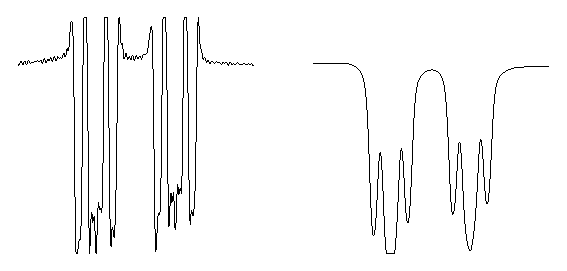
\epsfig{file=apodH.eps,width=3in,angle=180}
\end{center}
\caption[Effet du filtrage numérique sur un spectre du \prot.]
{Effet filtrage numérique sur un spectre du \prot.
A gauche, le spectre non filtré, et à droite filtré par un filtre de type
Lorentz-Gauss (rétrécissement des raies).}
\label{fig:apodH}
\end{figure}

La figure \ref{fig:apodH} montre comment 
la résolution d'un spectre de \prot à été artificiellement améliorée au dépend 
du rapport S/B et de la forme des raies.
Dans le spectre de \carb de la figure \ref{fig:apodC}, le rapport S/B
a été amélioré au dépend de la largeur des raies.

\begin{figure}[hbt]
\begin{center}
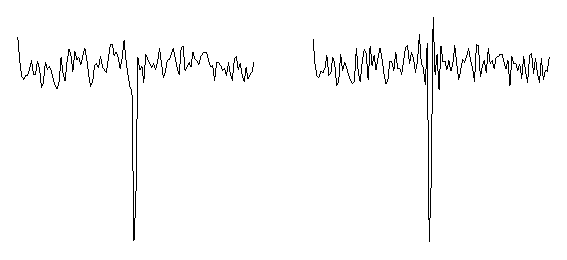
\epsfig{file=apodC.eps,width=3in,angle=180}
\end{center}
\caption[Effet filtrage numérique sur un spectre du \carb.]
{Effet du filtrage numérique sur un spectre du \carb.
A gauche, le spectre non filtré, et à droite filtré par un filtre de type
Lorentz (élargissement des raies).}
\label{fig:apodC}
\end{figure}

Le cas présenté figure \ref{fig:trunc} illustre la distorsion du spectre 
introduite par la troncature du signal.

\begin{figure}[hbt]
\begin{center}
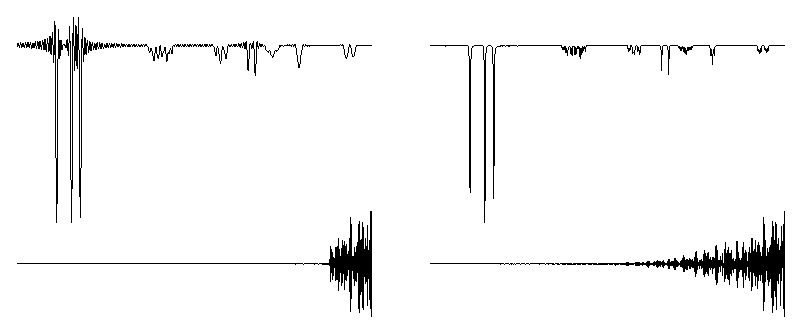
\epsfig{file=trunc.eps,width=5in,angle=180}
\end{center}
\caption[Effet de la troncature du \FID.]
{Effet de la troncature du \FID.
A gauche, le {\FID} non tronqué et le spectre correspondant.
A droite, le {\FID} tronqué et son spectre.}
\label{fig:trunc}
\end{figure}

Idéalement, le signal devrait être enregistré pendant un temps infini pour en 
recueillir l'intégralité. 
L'allongement du temps d'enregistrement entraîne une moindre 
efficacité de l'amélioration du rapport S/B par accumulation, une diminution du rapport 
S/B de chaque signal pris individuellement et enfin nécessite un volume de stockage du 
spectre important. 
Le temps d'enregistrement du signal, noté $\Delta t$, est déterminé par la 
largeur spectrale et par le nombre d'échantillons à enregistrer. Il se peut que l'amplitude 
du signal au temps $t = \Delta t$, proportionnelle à $\exp(-\Delta t/T_2^*)$
reste importante par rapport 
à l' amplitude initiale.
Le signal dont on calcule la TF est alors une fonction 
exponentielle décroissante tronquée et les raies du spectres ne seront plus de forme 
lorentzienne.

Déterminer la TF d'un signal $s(t)$ tronqué revient à calculer 
\begin{equation}
S(\Oms) = \int_0^{\Delta t} \exp(-i \Oms t). s(t) \, dt
\end{equation}
A titre d'exemple, si le signal est caractérisé par un $T_2^*$ infiniment long et une phase 
nulle, $s(t) = \exp(i \omzeros t)$ alors,
\begin{eqnarray}
S(\Oms) & = & \int_0^{\Delta t} \exp(-i t (\Oms - \omzeros)) d\Oms \\
& = & \frac{i}{\Oms - \omzeros} \left[ \exp(-i t(\Oms-\omzeros))\right]_0^{\Delta t} \\
& = & \frac{i}{\Oms - \omzeros} (\exp(i \Delta t (\Oms-\omzeros))-1)
\end{eqnarray}

Si on pose $u = \Delta t (\Oms -\omzeros)$ alors la partie réelle de 
$S(\Oms)$ vaut $\Delta t . \sin(u)/u$. 
Le spectre correspondant est tracé figure \ref{fig:sinc}, avec $\omzeros = 0$.
Cette fonction est centrée sur $\Oms = \omzeros$ et est significativement
différente d'une raie lorientzienne en absorption. 
La raie qui serait idéalement fine en l'absence de troncature 
a maintenant une largeur définie 
entre les points A et B, correspondant aux premières valeurs nulles de sin(u)/u, 
c'est-à-dire à $u = \pm\pi$. 
La largeur de la raie $\delta\Oms$ est alors telle que $\Delta t.\delta\Oms = 2 \pi$,
égale à la résolution numérique du spectre.
La raie est d'autant plus large que $\Delta t$ est court.

\begin{figure}[hbt]
\begin{center}
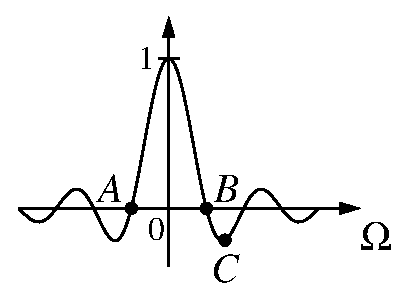
\epsfig{file=sinc.eps,width=3in}
\end{center}
\caption{Effet sur un spectre de la troncature du signal temporel.}
\label{fig:sinc}
\end{figure}

Qualitativement $\Delta t$ et $T_2^*$ 
jouent des rôles similaires puisque raccourcir le temps pendant lequel le signal a une 
intensité appréciable entraîne un élargissement des raies et une diminution de leur 
hauteur.
Toutefois, la relaxation n'introduit ni "pied" négatif dans le spectre ni de maxima 
secondaires. L'intensité de la première excursion négative (point C, figure \ref{fig:sinc}) 
est calculée pour $u = 3\pi/2$ et vaut $-2/3\pi = -0.212$, 
relativement à l'intensité du maximum principal. 
Des pics de faible intensité situés au voisinage du pic principal 
seront masqués par la distorsion de 
la ligne de base engendrée par la troncature.

Le cas analysé ici est un cas extrême, l'autre cas extrême est celui où $T_2^*$ est très 
inférieur à $\Delta t$. 
Au moment où cesse l'acquisition du signal il n'y a alors plus de signal 
mesurable (sauf du bruit) et la troncature n'a plus d'effet ni sur la largeur des raies ni sur 
leur forme. 
Dans les cas intermédiaires la troncature introduit un élargissement des raies 
et l'apparition de maxima secondaires positifs et négatifs, mais d'intensité relative plus 
faible qu'en l'absence de relaxation.

\section{L'apodisation}
Pour couper le pied (apodiser) négatif des raies issues d'un signal tronqué et restaurer leur 
forme lorentzienne, il suffit de multiplier $s(t)$ par une fonction exponentielle 
décroissante $\exp(-t/\tau)$ avec $\tau > 0$ (Figure \ref{fig:apodC}).
Le signal $s(t) = \exp(-t/T_2^*).\exp(i \omzeros t)$ devient 
$\exp(-t.(1/T_2^* + 1/\tau)).\exp(i \omzeros t)$. 
Tout se passe comme si $T_2^*$ avait été diminué, l'amortissement du 
signal étant caractérisé par un paramètre $\lambda$ tel que 
\begin{equation}
1/\lambda = 1/T_2^* + 1/\tau
\end{equation}
La largeur à mi-hauteur $\Delta\nu_{1/2}$ d'une raie lorentzienne est reliée à 
$\lambda$ par $\Delta\nu_{1/2} = 1/\pi\lambda$, 
l'apodisation par une fenêtre exponentielle décroissante $\exp(-t/\tau)$ élargit donc les raies 
de $1/\pi\lambda$ Hertz. 
Si $\tau$ est choisi suffisamment grand pour que le signal soit pratiquement 
nul à $t = \Delta t$, les raies du spectre ne présentent plus d'oscillations à leur base mais leur 
élargissement diminue la résolution du spectre.

L'apodisation n'est pas sans répercussion sur le rapport signal sur bruit du spectre.
Le bruit reste d'intensité constante de $t=0$ à $t=\Delta t$.
Puisque le signal issu de l'échantillon décroît au cours du temps, on peut
dire que le rapport signal sur bruit décroît aussi au cours de l'enregistrement.
Multiplier le signal par une exponentielle décroissante peut totalement
annuler le bruit lorsque $t$ est voisin de $\Delta t$.
Cette même opération atténue aussi le signal.
Il est possible de montrer que le rapport signal sur bruit est optimisé
lorsque qu'on apodise le signal avec $\tau = T_2^*$.

Lorsque le rapport signal sur bruit est important il est possible d'en tirer parti pour 
améliorer la résolution du spectre. 
Si le signal est multiplié par une fonction 
exponentielle croissante $\exp(t/\tau)$, ($\tau > 0$) 
la largeur à mi-hauteur des raies est diminuée de 1/$\pi\tau$ 
(en l'absence de troncature) et le rapport signal sur bruit diminue. 
En considérant que 
toutes les raies du spectre ont le même $T_2^*$, multiplier le signal par $\exp(t/T_2^*)$ 
compense complètement l'effet de la relaxation et les raies atteignent leur largeur 
minimale de l'ordre de $1/\Delta t$.
L'effet sur le rapport signal sur bruit peut alors être catastrophique.
Il faut donc multiplier à nouveau le signal temporel par une fonction
qui va atténuer fortement la fin
du signal tout en laissant le début le plus intact possible.
Cela se réalise par exemple avec une fonction gaussienne. 
Cette dernière va contribuer
bien entendu à élargir les raies, mais de manière contrôlable, tout en leur
donnant une forme assez complexe.
La transformation du signal résultante (Lorentz-Gauss) est pratiquement utilisée pour
faciliter la séparation de signaux de fréquences extrêmement voisines
(Figure \ref{fig:apodH}).
L'utilisateur doit rechercher un compromis entre les différentes
options qui lui permettent de modifier la résolution, la forme des raies, le
rapport sur bruit, et ceci en fonction du signal disponible et de la nature
des informations recherchées dans le spectre.

\section{Le zero filling}
La technique du "remplissage avec des zéros" contribue à l'amélioration de séparation 
entre raies de fréquences voisines, et consiste à faire suivre par des valeurs numériques 
nulles les valeurs du signal numérisé du signal avant transformée de Fourier. 
L'intérêt de cette manipulation est illustré figure \ref{fig:zerofill}, 
où le spectre $a$ est obtenu par TF d'un signal 
composé de 4094 valeurs complexes. 
Le signal en question est "allongé" à l'aide zéros 
jusqu'à obtenir un signal de 16384 valeurs complexe, les 12288 derniers étant nulles. 
Le spectre de droite, composé de 16384 points complexes présente des détails fins invisibles dans 
celui de gauche. Seule une petite région spectrale est représentée.

\begin{figure}[hbt]
\begin{center}
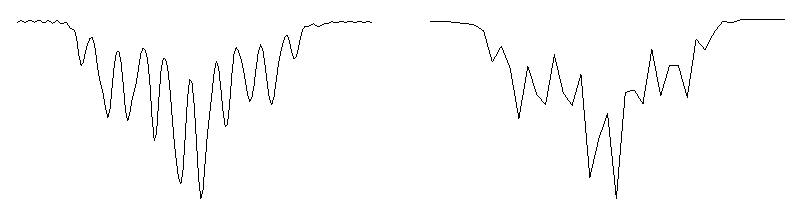
\epsfig{file=zerofill.eps,width=5in,angle=180}
\end{center}
\caption[Effet du zero-filling.]
{A gauche, spectre sans zero filling avant TF. A droite, le signal temporel a été allongé 4 fois.}
\label{fig:zerofill}
\end{figure}

Le zero filling a pour but d'augmenter artificiellement la résolution numérique
puisque la largeur spectrale ne change pas et que le nombre de points qui définit
la taille du spectre augmente (ce nombre est égal au nombre de valeurs du signal temporel).
Le zero filling fournit une interpolation de $S(\Oms)$ entre les valeurs issues d'une TF
sans zero filling.
Il est généralement admis que multiplier la taille du spectre par un facteur 2 apporte 
une amélioration utile, et qu'utiliser un facteur plus important n'apporte
pas d'amélioration sensible.

\section{Le programme de phases}
\label{sec:progphaseft}

Un spectre enregistré par la méthode impulsionnelle présentée dans ce chapitre peut présenter
des pics à des positions inattendues, et dont l'intensité
dépend de la qualité des dispositifs électroniques qui constituent
la chaîne d'acquisition du signal.
Un artefact exactement situé au milieu du 
spectre ($\Oms = 0$) est appelé pic axial et un artefact symétrique du pic réel par rapport au pic 
axial est appelé "fantôme de quadrature" ($\Oms = - \omzeros$)
pour une raison qui apparaîtra ci-après.
L'enregistrement de signaux successifs où les 
phases de l'impulsion et du récepteur sont modifiées entre chaque séquence excitation - 
détection permet l'élimination de ces artefacts. 
Le concept de programme de phase introduit ici sera 
réexaminé dans le cadre plus général des expériences multi--impulsionnelles.

L'analyse du programme de phase associé à une expérience de RMN
consiste à étudier comment varie le signal en 
fonction de la phase de l'impulsion (ou des impulsions) qui l'a créé. 
Dans l'expérience élémentaire "excitation - détection", 
il a été signalé qu'une augmentation de la phase de l'impulsion entraîne une 
augmentation identique de l'angle que fait la composante transversale
de l'aimantation avec l'axe $OX$.
En identifiant signal complexe et aimantation transversale dans le référentiel tournant,
augmenter de $\Delta \phi$ la phase de l'impulsion revient à 
multiplier $s(t)$ par $\exp(i.\Delta\phi)$. 
Ainsi si $\Delta\phi = \pi/2$, alors $s(t)$ devient $i.s(t)$. 

Un détecteur idéal est censé délivrer une tension nulle en l'absence de grandeur à 
mesurer. 
Dans la réalité, une tension continue, ou tension de décalage, 
est présente à la sortie du (ou des) détecteur(s). 
On notera $\epsilon$ cette tension et $s(t,\phi = 0)$ 
le "vrai" signal complexe en supposant 
que la phase $\phi$ de l'impulsion utilisée est nulle; 
le signal complexe mesuré est alors  $s(t, 0) + \epsilon = s'(t, 0)$. 
Le tableau \ref{tab:phasea} résume les valeurs du signal complexe 
mesuré en fonction de la phase de l'impulsion.

\begin{table}
\caption{Variation du signal en fonction de la phase de l'impulsion, 
effet d'une composante continue}
\label{tab:phasea}
\begin{center}
\begin{tabular}[hbt]{crcl}
\hline
Phase    &                     & $s(t)$ &          \\ \hline
$0$      &  $1.s(t,0) + \epsilon$ & = & $s'(t,0)$ \\
$\pi/2$  &  $i.s(t,0) + \epsilon$ & = & $s'(t,\pi/2)$ \\
$\pi$    &   $-s(t,0) + \epsilon$ & = & $s'(t,\pi)$ \\
$-\pi/2$ & $-i.s(t,0) + \epsilon$ & = & $s'(t,-\pi/2)$ \\
\hline
\end{tabular}
\end{center}  
\end{table}

Si on additionne $s'(t,0)$ et l'opposé de $s'(t,\pi)$ on constate l'annulation du terme 
d'erreur et l'addition constructive des signaux vrais : 
$s'(t,0) - s'(t,\pi) = 2.s(t,0)$. 
Ce résultat est général si on considère les signaux issus de deux impulsions de 
phases différent de $\pi$.

L'amplitude de la composante du signal ayant une fréquence nulle 
c'est-à-dire $S(\Oms = 0)$ est calculée par selon la définition de la TF : 
\begin{equation}
		S(0) = \intzp s(t).\exp(i.0.t) \, dt = \intzp s(t) \, dt
\end{equation}
qui correspond à la définition de la moyenne du signal. 
Superposer une composante $\epsilon$
continue au signal (de moyenne non nulle par définition) 
revient à modifier la valeur de 
$S(\Oms = 0)$ et donc à introduire dans le spectre un pic axial.
Utiliser $s'(t,0) - s'(t,\pi) = 2.s(t,0)$ au lieu
de $2(s(t,0)+\epsilon)$ permet donc d'éliminer le pic axial.

En supposant maintenant qu'il n'y a pas d'erreur de décalage mais une différence de gain 
d'amplification des signaux $s_x(t)$ et $s_y(t)$ issus des deux démodulateurs, le signal 
complexe effectivement enregistré lorsque la phase de l'impulsion est nulle s'écrit :
\begin{equation}
s'(t,0) = s_x(t,0).(1+\delta) + i.s_y(t,0).(1-\delta) 
\end{equation}
où $1+\delta$ et $1-\delta$ sont les gains relatifs des deux chaînes d'amplification. 
Ces gains sont en principe ajustés de façon à valoir 1 et 1 
mais des variations peuvent apparaître au cours du temps. 
L'effet de la dissymétrie entre les deux canaux de réception est mise en évidence 
en écrivant 
\begin{equation}
s'(t,0) = 1.(s_x(t,0) + i.s_y(t,0)) + \delta.(s_x(t,0) - i.s_y(t,0)) 
\end{equation}
si, pour simplifier, on omet le terme de relaxation et de phase du signal :
\begin{eqnarray}
s_x(t,0) &=& \cos(\omzeros t) \\
s_y(t,0) &=& \sin(\omzeros t)
\end{eqnarray}
alors :
\begin{equation}
		s'(t,0) = 1.\exp(i \omzeros t) + \delta.\exp(-i \omzeros t)
\end{equation}
la partie réelle de la TF de $s'(t,0)$ présente une raie 
d'intensité relative 1 à la pulsation $\omzeros$ et une autre raie, 
le "fantôme de quadrature", à la 
pulsation $-\omzeros$ et d'intensité relative $\delta$. 
On peut considérer que l'apparition de ce pic non 
voulu est lié à une incapacité du détecteur à distinguer parfaitement les fréquences 
positives des fréquences négatives lorsque les canaux de réception sont non 
symétriques. 
A l'extrême si un des canaux vient à ne plus fonctionner (gain nul), alors $\delta$ 
vaut 1 ou -1 : le pic attendu et son image de quadrature ont la même intensité, ce
qui correspond à une détection à une détection sur un seul canal et donc
à une indétermination du signe des fréquences.
 
Le tableau \ref{tab:phaseb} indique pour les diverses valeurs de phase $\phi$ de l'impulsion 
ce qu'est le signal enregistré $s'(t,\phi)$ en 
fonction de s(t,0) et de s*(t,0), avec 
\begin{eqnarray}
s(t,0) & = & s_x(t,0) + i.s_y(t,0) \\
s^*(t,0) & = & s_x(t,0) - i.s_y(t,0)
\end{eqnarray}

\begin{table}
\caption{Variation du signal en fonction de la phase de l'impulsion, 
effet d'une erreur de quadrature}
\label{tab:phaseb}
\begin{center}
\begin{tabular}[hbt]{cc}
\hline
$\phi$    &                      $s'(t,\phi)$           \\ \hline
$0$      &  $1.s(t,0)  + \delta.s^*(t,0)$ \\
$\pi/2$  &  $i.s(t,0) -i \delta.s^*(t,0)$ \\
$\pi$    &   $-s(t,0)  - \delta.s^*(t,0)$ \\
$-\pi/2$ & $-i.s(t,0) +i \delta.s^*(t,0)$ \\
\hline
\end{tabular}
\end{center}  
\end{table}


Ainsi augmenter $\phi$ de $\pi/2$ revient à multiplier le terme $s(t,\phi)$ par $i$ 
et le terme $s^*(t,\phi)$ par $-i$ : 
\begin{equation}
s'(t,\phi+\pi/2) = i . s(t,\phi) - \delta . i . s^*(t,\phi)
\end{equation}
Dans un cas plus général on aurait :
\begin{equation}
s'(t,\phi+\Delta \phi) = \exp(i \Delta \phi) . s(t,\phi) + 
\delta.\exp(i.-\Delta \phi) . s^*(t,\phi)
\end{equation}

Pour éliminer l'erreur de quadrature il suffit d'additionner 
$s'(t,0)$ et $-i . s'(t,\pi/2)$ :
\begin{eqnarray}
    s'(t,0)     & = & s(t,0) + \delta.s^*(t,0) \\
- i.s'(t,\pi/2) & = & s(t,0) - \delta.s^*(t,0)
\end{eqnarray}
et leur somme vaut $2.s(t,0)$ indépendamment de $\delta$.

On peut montrer que si le déphaseur du récepteur en quadrature (figure \ref{fig:spectrob})
effectue un déphasage différent de $\pi/2$, une erreur de quadrature se produit,
identique à celle qui résulte du déséquilibre entre les deux voies de réception.

Pour éliminer simultanément l'erreur de 
décalage et de quadrature ($\delta$ et $\epsilon$ non nuls) 
un calcul analogue à celui présenté ci-dessus indique qu'il faut calculer 
la somme :
\begin{equation}
	s'(t,0) - i.s'(t,\pi/2) - s'(t,\pi) + i.s'(t,-\pi/2)
\end{equation}
qui vaut $4.s(t,0)$ indépendamment de $\delta$ et de $\epsilon$. 
La notion de phase du récepteur permet de formaliser cette manipulation des signaux. 
Pour additionner de façon cohérente les signaux, 
c'est-à-dire pour renforcer les vrais signaux et annuler les 
imperfections il faut augmenter successivement la phase de l'impulsion par pas de $\pi/2$ et 
augmenter identiquement la phase du récepteur : 
augmenter la phase du récepteur 
de $\pi/2$ revient à multiplier le signal complexe par $\exp(-i.\pi/2) = -i$. 
Pour supprimer toute confusion due au vocabulaire il faudrait parler de 
"déphasage du signal après acquisition" plutôt que de phase du récepteur. 
La multiplication du signal par $-i$ compense la multiplication du 
signal complexe par $i$ introduite par l'augmentation  de $\pi/2$ de la phase de l'impulsion. 
Les signaux vrais sont les seuls à être multipliés par $i$, 
ce sont les seuls à être additionnés de façon constructive. 
Dans le cas de l'expérience impulsion -- détection traitée jusqu'ici, la 
relation entre phase du récepteur $\phi_R$ et phase de l'impulsion (ou phase de l'émetteur) 
est donc :
\begin{equation}
\Delta \phi_R = \Delta \phi.
\end{equation}

En utilisant les conventions introduites dans la table \ref{tab:phase},
le programme de phase qui vient d'être décrit se note :
\begin{eqnarray}
  \phi & = & (x, y, -x, -y) \\
\phi_R & = & (x, y, -x, -y)
\end{eqnarray}
l'élimination des pics indésirables n'étant réalisée qu'après addition de quatre signaux. 
La mise en {\oe}uvre pratique du changement de phase du récepteur se limite en fait à des 
additions ou à des soustractions de signaux réels : si $s'(t)$ est écrit comme $s_x'(t) + i.s_y'(t)$ 
les parties réelles et imaginaires des termes à sommer sont données dans le tableau \ref{tab:phasec}.

\begin{table}
\caption{Phase du récepteur}
\label{tab:phasec}
\begin{center}
\begin{tabular}[hbt]{ccc}
\hline
terme    &  partie réelle & partie imaginaire           \\ \hline
$s'(t)   $ & $s_x'(t) $ & $s_y'(t)$  \\
$-i.s'(t)$ & $s_y'(t) $ & $-s_x'(t)$ \\
$-s'(t)  $ & $-s_x'(t)$ & $-s_y'(t)$ \\
$i.s'(t) $ & $-s_y'(t)$ & $s_x'(t)$  \\
\hline
\end{tabular}
\end{center}  
\end{table}

Il suffit donc après chaque numérisation des signaux $s_x'(t)$ et $s_y'(t)$ de sommer les 
valeurs obtenues, munies du signe requis, vers la partie réelle ou vers la partie 
imaginaire du signal total, comme indiquée dans le tableau \ref{tab:phasec}.

La notion de programme de phase sera réexaminée au paragraphe \ref{sec:progphasedensite} 
dans le cadre du formalisme de la matrice densité.

